\documentclass{homework}

\title{Homework 6}
\author{Kevin Evans}
\studentid{11571810}
\date{October 14, 2020}
\setclass{Physics}{341}
\usepackage{amssymb}
\usepackage{mathtools}

\usepackage{amsthm}
\usepackage{amsmath}
\usepackage{slashed}
\usepackage{relsize}
\usepackage{threeparttable}
\usepackage{float}
\usepackage{booktabs}
\usepackage{boldline}
\usepackage{changepage}
\usepackage{physics}
\usepackage[inter-unit-product =\cdot]{siunitx}
\usepackage{setspace}

\usepackage[makeroom]{cancel}
%\usepackage{pgfplots}

\usepackage{enumitem}
\usepackage{times}

\usepackage{calligra}
\DeclareMathAlphabet{\mathcalligra}{T1}{calligra}{m}{n}
\DeclareFontShape{T1}{calligra}{m}{n}{<->s*[2.2]callig15}{}
\newcommand{\scriptr}{\mathcalligra{r}\,}
\newcommand{\boldscriptr}{\pmb{\mathcalligra{r}}\,}

\begin{document}
	\maketitle
	\begin{enumerate}
		\item From the method of images, the arrangement is equivalent to a $-q$ charge at $-d$ and a $q$ charge at $-2d$. Summing these, \begin{align*}
			\bvec{F} & = q \sum_i \bvec{E}_i \\
				& = \frac{q^2}{4 \pi \epsilon_0} \left[\frac{1}{d^2} - \frac{1}{(2d)^2} + \frac{1}{(3d)^2}\right] \uvec{z} \\
				& = \frac{31q^2}{144 \pi \epsilon_0 d^2} \uvec{z}
		\end{align*}
	
		\item There would be 3 other charges: \begin{center}
			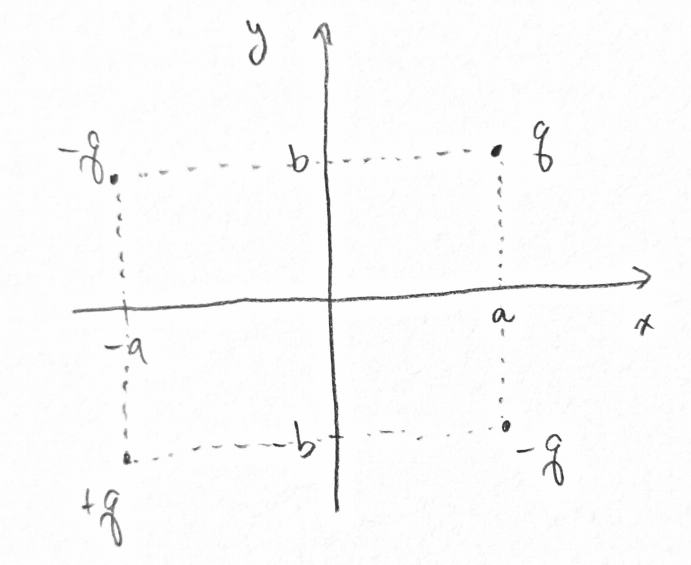
\includegraphics[width=0.5\linewidth]{hw6_2}
		\end{center}
		Summing the three point charge potentials,\begin{align*}
			V(x, y) & = \frac{q}{4 \pi \epsilon_0} \bigg[
				\frac{1}{\sqrt{\left(x - a\right)^2 + \left(y - b\right)^2}}
				+ \frac{1}{\sqrt{\left(x + a\right)^2 + \left(y + b\right)^2}} \\
			& \qquad
				- \frac{1}{\sqrt{\left(x + a\right)^2 + \left(y - b\right)^2}}				
				- \frac{1}{\sqrt{\left(x - a\right)^2 + \left(y + b\right)^2}}
			\bigg]
		\end{align*}
		Summing the forces on $q$, \begin{align*}
			\bvec{F} & = \frac{q^2}{4 \pi \epsilon_0} \left[-\frac{1}{4a^2} \uvec{x} - \frac{1}{4b^2} \uvec{y} + \frac{1}{\left( \sqrt{ 4a^2 + 4b^2 } \right)^2} \left(\frac{2a}{\sqrt{4a^2 + 4b^2}} \uvec{x} + \frac{2b}{\sqrt{4a^2 + 4b^2}} \uvec{y}\right) \right] \\
				& = \frac{q^2}{4 \pi \epsilon_0} \left[
					\left( \frac{2a}{\left(4a^2 + 4b^2 \right)^{3/2}} - \frac{1}{4a^2} \right) \uvec{x}
					+ \left( \frac{2b}{\left(4a^2 + 4b^2 \right)^{3/2}} - \frac{1}{4b^2} \right) \uvec{y}
				\right]
		\end{align*}
		To bring $q$ from infinity, the work required \begin{align*}
			W & = q \sum_i V_i \\
				& = \frac{q^2}{4 \pi \epsilon_0} \Bigg[\frac{1}{\sqrt{\left(x + a\right)^2 + \left(y + b\right)^2}} \\
				& \qquad
				- \frac{1}{\sqrt{\left(x + a\right)^2 + \left(y - b\right)^2}}				
				- \frac{1}{\sqrt{\left(x - a\right)^2 + \left(y + b\right)^2}}
				\Bigg]_{x=a,y=b} \\
				& = \frac{q^2}{4 \pi \epsilon_0} \left[ \frac{1}{\sqrt{4a^2 + 4b^2}} - \frac{1}{\sqrt{4a^2}} - \frac{1}{\sqrt{4b^2}} \right]
		\end{align*}
		
		The method of images seems to work with angles where $360^\circ / n$, where $n = 1, 2, 3...$?
		
%		\pagebreak
		\item \begin{enumerate}
			\item Since the potential must be periodic-ish in $x$, the assumed form of the potential is \begin{align*}
				V(x, y) & = \left(Ae^{ky} + Be^{-ky}\right) \left(C \sin kx + D \cos kx\right)
				\intertext{Since $V(0, y) = 0 \implies D = 0$, and since it's zero at $x=a$, the wavenumber can be found}
				V(x, y) & = \left(Ae^{ky} + Be^{-ky}\right) C \sin(\frac{n \pi}{a}x)
				\intertext{Since $V(x, 0) = 0$, then $A = -B$ and we can replace the exponentials with a $\sinh$ and use a single constant $C'$,}
				V(x, y) & = C' \sinh( \frac{n \pi}{a} y ) \sin( \frac{ n \pi}{a} x )
				\intertext{Since any linear combination is a solution, the general solution has the form}
				V(x, y) & = \sum_n C_n \sinh( \frac{n \pi}{a} y ) \sin( \frac{ n \pi}{a} x )
				\intertext{Applying Fourier's trick at the $y=b$ boundary to find the coefficients,}
				\int_0^a V_0 (x) \sin( \frac{n' \pi x}{a} ) \dd{x} & = \sum_n C_n \int_0^a \sinh( \frac{n \pi}{a} b ) \sin( \frac{ n \pi }{a} x) \sin(\frac{n' \pi }{a} x) \dd{x} \\
					& = C_n \sinh( \frac{n \pi}{a} b) \frac{a}{2} \\
				C_n & = \frac{2}{a} \left( \frac{1}{\sinh(n \pi b / a)} \right) \int_0^a V_0(x) \sin( \frac{n \pi x}{a} ) \dd{x}
			\end{align*}
			\item For $V_0(x) = \beta x$, \begin{align*}
				C_n & = \frac{2\beta}{a} \left( \frac{1}{\sinh(n \pi b / a)} \right) \int_0^a \sin( \frac{n \pi x}{a} ) x \dd{x} \\
					& = \frac{2 \beta}{a} \left( \frac{1}{\sinh(n \pi b / a)} \right) \left( -\frac{a^2 \cos(\pi n)}{\pi n} \right) && \leftarrow \text{Used WolframAlpha} \\
					& = - \frac{2 \beta a}{\pi n} \frac{\cos( \pi n)}{\sinh( n \pi b / a)}
				\intertext{Using this $C_n$ in $V(x, y)$,}
				V(x, y) & =  - \sum_n \frac{2 \beta a}{\pi n} \frac{\cos( \pi n)}{\sinh( n \pi b / a)} \sinh( \frac{n \pi}{a} y ) \sin( \frac{ n \pi}{a} x )
			\end{align*}
		
			\pagebreak
			Plotting this to check the result and it seems to resemble the boundary conditions (for $a=5$, $b=4$, $\beta=1$, $N=20$):
			% TODO: \usepackage{graphicx} required
			\begin{center}
				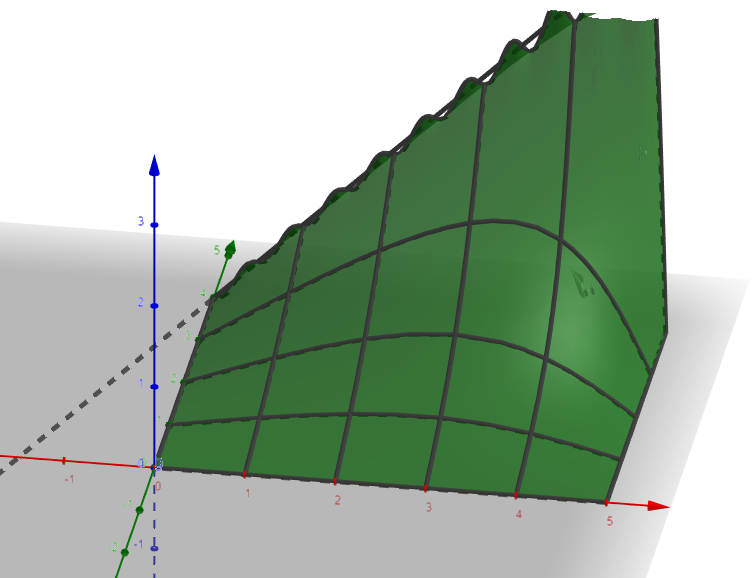
\includegraphics[width=0.7\linewidth]{hw6_3}
			\end{center}
			
		\end{enumerate}
	
		\item From the geometry, it seems like the $x$ and $y$ directions will have a periodic term, and the $z$ direction will have an exponential. The potential will be in the form of \begin{align*}
			V(x, y, z) & = \left(A \sin kx + B \cos kx\right)
				\left(C \sin l y + D \cos ly\right)
				\left(E e^{m z} + F e^{-mz}\right)
			\intertext{Applying the $x$ boundary conditions, $V(0, y, z) = V(a, y, z) = 0$, then $B=0$ and $k$ can be determined. Similarly for $y$, $D=0$ and $l$ can be found. In $z$, $E=-F$ at $z=0$ and additionally, $m$ can be written in terms of $k$ and $l$ as well (arising from the separable DE). The form becomes}
			V(x, y, z) & = C' \sin( \frac{n \pi}{a} x) \sin( \frac{m \pi}{b} y) \sinh(\sqrt{k^2 + l^2} z)
			\intertext{Applying the orthogonality of sines, } 
			V(x, y, z) & = \sum_n \sum_m C_{n,m} \sin( \frac{n \pi}{a} x) \sin( \frac{m \pi}{b} y) \sinh(\sqrt{k^2 + l^2} z)
			\intertext{At the $z=c$ boundary, }
			V(x, y, c) & = \sum_n \sum_m C_{n,m} \sin( \frac{n \pi}{a} x) \sin( \frac{m \pi}{b} y) \sinh(\sqrt{k^2 + l^2} c) \\
			V_0 \int_0^a \int_0^b \sin(\frac{n' \pi}{a}x) \sin(\frac{m' \pi}{b} y) \dd{y} \dd{x} & = \int_0^a \int_0^b \sum_n \sum_m C_{n,m} \sin( \frac{n \pi}{a} x) \sin( \frac{m \pi}{b} y) \sinh(\sqrt{k^2 + l^2} c) \\
				& \qquad \times \sin(\frac{n' \pi}{a}x) \sin(\frac{m' \pi}{b} y) \dd{y} \dd{x}
			\intertext{Filtering out only the $n=n'$ and $m=m'$ cases (Fourier's trick) and evaluating the integrals, for odd $n$ and $m$,}
			C_{n, m} & = \frac{4 V_0}{ab \sinh(\sqrt{k^2 + l^2} c)} \left(\frac{2a}{\pi n}\right) \left(\frac{2b}{\pi m}\right) \\
				& = \frac{16 V_0}{\pi^2 nm \sinh(\sqrt{k^2 + l^2} c) }
			\intertext{Putting this all together in the general equation and substituting $k$ and $l$ into the $\sinh$,}
			V(x, y, z) & = \frac{16V_0}{\pi^2} \sum_{n, m=1,3,5...} \frac{1}{nm \sinh(\pi \sqrt{(n/a)^2 + (m/b)^2} c)} \\
				& \qquad \times \sinh(\pi \sqrt{(n/a)^2 + (m/b)^2} z)  \sin( \frac{n \pi}{a} x) \sin( \frac{m \pi}{b} y)
		\end{align*}
	
		
		\item On the ground plane at $y=a$, the normal direction is $\hat{y}$, the induced charge is found through \begin{align*}
			\sigma(x) & = - \epsilon_0 \eval{ \pdv{V(x, y)}{y} }_{y=a} \\
				& = -\frac{4V_0}{\pi \epsilon_0} \sum_{n=1,3...} \pdv{y} \frac{1}{n} \frac{\sinh(n \pi x/a)}{\sinh(n \pi b / a)} \sin(n \pi y / b) \eval_{y=a}\\
				& = -\frac{4V_0}{\epsilon_0 b} \sum_{n=1,3...} \frac{\sinh(n \pi x/a)}{\sinh(n \pi b / a)} \cos(n \pi a / b) \\
		\end{align*}
	\end{enumerate}
\end{document}